\documentclass[
	12pt,
	]{article}
		\usepackage{xcolor}
			\usepackage[dvipsnames]{xcolor}
			\usepackage[many]{tcolorbox}
		\usepackage{changepage}
		\usepackage{titlesec}
		\usepackage{caption}
		\usepackage{mdframed}
		\usepackage{mathtools, amssymb, amsfonts, amsthm, bm,amsmath} 
		\usepackage{array, tabularx, booktabs}
		\usepackage{graphicx,wrapfig, float, caption}
		\usepackage{tikz,physics,cancel, siunitx, xfrac}
		\usepackage{graphics, fancyhdr}
		\usepackage{lipsum}
		\usepackage{xparse}
		\usepackage{thmtools}
		\usepackage{mathrsfs}
		\usepackage{undertilde}
		\usepackage{dutchcal}
		\usepackage{tikz}
		\usepackage{fullpage}
		\usepackage[labelfont=bf]{caption}
	\newcommand{\td}{\text{dim}}
	\newcommand{\tvw}{T : V\xrightarrow{} W }
	\newcommand{\ttt}{\widetilde{T}}
	\newcommand{\ex}{\textbf{Example}}
	\newcommand{\aR}{\alpha \in \mathbb{R}}
	\newcommand{\abR}{\alpha \beta \in \mathbb{R}}
	\newcommand{\un}{u_1 , u_2 , \dots , n}
	\newcommand{\an}{\alpha_1, \alpha_2, \dots, \alpha_2 }
	\newcommand{\sS}{\text{Span}(\mathcal{S})}
	\newcommand{\sSt}{($\mathcal{S}$)}
	\newcommand{\la}{\langle}
	\newcommand{\ra}{\rangle}
	\newcommand{\Rn}{\mathbb{R}^{n}}
	\newcommand{\R}{\mathbb{R}}
	\newcommand{\Rm}{\mathbb{R}^{m}}
	\usepackage{fullpage, fancyhdr}


	\usepackage{mathtools}
	\DeclarePairedDelimiter{\norm}{\lVert}{\rVert}
	\newcommand{\vectorproj}[2][]{\textit{proj}_{\vect{#1}}\vect{#2}}
	\newcommand{\vect}{\mathbf}
	\newcommand{\uuuu}{\sum_{i=1}^{n}\frac{<u,u_i}{<u_i,u_i>} u_i}
	\newcommand{\B}{\mathcal{B}}
	\newcommand{\Ss}{\mathcal{S}}
	
	\newtheorem{theorem}{Theorem}[section]
	\theoremstyle{definition}
	\newtheorem{corollary}{Corollary}[theorem]
	\theoremstyle{definition}
	\newtheorem{lemma}[theorem]{Lemma}
	\theoremstyle{definition}
	\newtheorem{definition}{Definition}[section]
	\theoremstyle{definition}
	\newtheorem{Proposition}{Proposition}[section]
	\theoremstyle{definition}
	\newtheorem*{example}{Example}
	\theoremstyle{example}
	\newtheorem*{note}{Note}
	\theoremstyle{note}
	\newtheorem*{remark}{Remark}
	\theoremstyle{remark}
	\newtheorem*{example2}{External Example}
	\theoremstyle{example}
	
	\title{PHYS 241 Lab 3.}
	\titleformat*{\section}{\LARGE\normalfont\fontsize{12}{12}\bfseries}
	\titleformat*{\subsection}{\Large\normalfont\fontsize{10}{15}\bfseries}
	\author{Mihail Anghelici 260928404 \\ Section  22524 Thursday\\ \\ Experiment performed with Guillaume Payeur}
	\date{March 12, 2020}
	
	\relpenalty=9999
			\binoppenalty=9999
		
			\renewcommand{\sectionmark}[1]{%
			\markboth{\thesection\quad #1}{}}
			
			\fancypagestyle{plain}{%
			  \fancyhf{}
			  \fancyhead[L]{\rule[0pt]{0pt}{0pt} Lab $3$} 
			  \fancyhead[R]{\small Mihail Anghelici $260928404$} 
			  \fancyfoot[C]{-- \thepage\ --}
			  \renewcommand{\headrulewidth}{0.4pt}}
			\pagestyle{plain}
			\setlength{\headsep}{1cm}
	\captionsetup{margin =1cm}
	\begin{document}
	\maketitle
		\section*{Question 1.}
			\begin{figure}[H]
				\centering
				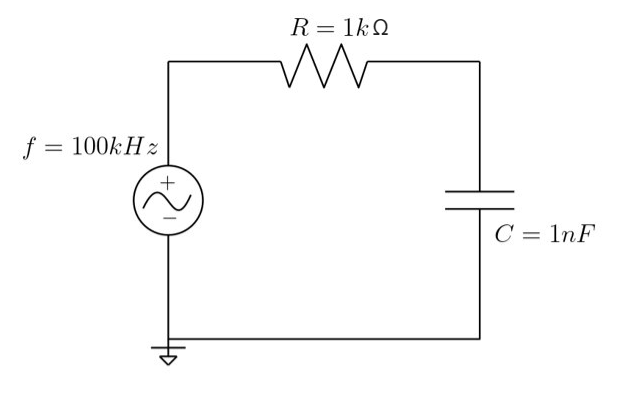
\includegraphics[width=0.6\linewidth]{PHYS241_Lab3_P1.png}
				\captionsetup{margin=1cm}
				\caption{Low-Pass circuit for a $3 \ $dB point of $100 \ \si{\kilo\hertz}$.}
			\end{figure}
			\begin{gather*}
				f_{H} = 100 000 \ \si{\hertz} = \frac{1}{2\pi R C} = \frac{1}{2\pi 1000 \ \si{\ohm} C} \implies C = 1\cross 10^{-9} = 1 nF.
			\end{gather*}
			\begin{figure}[H]	
				\centering
				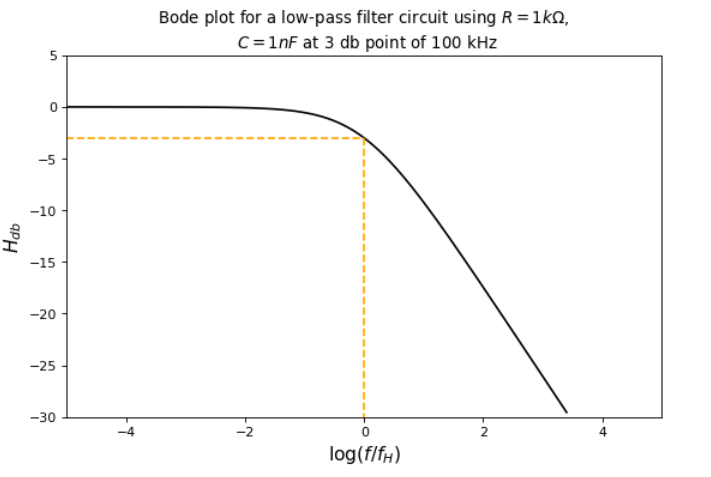
\includegraphics[width=0.9\linewidth]{phys241_lab3_picture1.png}
				\captionsetup{margin=1cm}
				\caption{Bode plot for low-pass filter circuit.The dotted lines indicate the $3$ db point.}
			\end{figure}
		\section*{Question 2.}
		In Experiment 1, the theoretical predicted values for $f_{H}$ and $\phi$ are found as follows
		\begin{align*}
			f_{H} &= \frac{1}{2\pi R C} = \frac{1}{2\pi 10000 \ \si{\ohm} \ 0.01 \ \si{\micro\farad}}\\
			&= 1591 \ \si{\kilo\hertz}.\\
			\phi &= \arctan(\omega C R) \qquad , \omega_{C} = 1/CR \\
			\implies \phi &= \arctan(1) = \pi / 4= 45 ^\circ.
		\end{align*}
		Experimentally it was found that $f_{H}  = 1470 \ \si{\kilo\hertz}$ and the phase angle was evaluated graphically using the difference tool between the two channel sine-waves , $\phi = 45 ^\circ$. The latter value is in excellent agreement with the theoretical value whilst the former has a considerable difference percentage. This difference is explained by the off-set present in the $V_C$ amplitude read on the scope compared to it's real amplitude. We noted that it was easier to measure the angle $\phi$ from the zero crossing compared to the peak separations since there's less visual fluctuation. Indeed, the $0$-crossing horizontal line is assumed to be perfectly linear, which is advantageous with respect to measuring the distance between two wave points at equal heights. 
		\section*{Question 3.}
			\begin{figure}[H]	
						\centering
						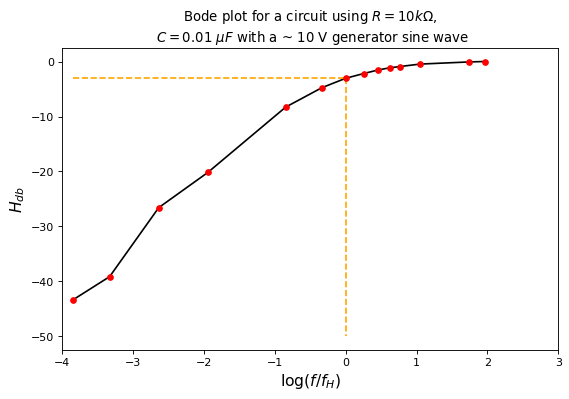
\includegraphics[width=0.9\linewidth]{phys241_lab3_picture2.png}
				\end{figure}
				
				\captionof{figure}{
										Bode plot for Experiment 2.The dotted lines indicate the $3$ db point. When compared to Figure 6 in  \textit{PHYS $241$ Signal Processing: Lab 3} manual, the plot is similar with respect to the dimensional limits, although is reflected with respect to the y-axis. It also looks less smooth in comparison. This lack of smoothness is explained by a lack of points taken in the range of $[-4,-2]$ on the x-axis. Another reason could be that some points withing that range have been miss-evaluated. 
				}
				
				\vspace{0.5cm}
		\section*{Question 4.}
			Experimentally it was found that the phase angle $\phi$ is $45 ^\circ$. 
				From Figure 3, we may immediately compute the angle $\phi$, 
						\begin{gather*}
							\text{Using R= 10 \ \si{\kilo\ohm} , C = 0.01 \ \si{\micro\farad} , we get} \\
							\phi = \arctan \left(\frac{1}{\omega RC}\right) = \arctan(-1) = -\pi/4.
						\end{gather*}
						The found angles are both in agreement with respect to their magnitude ,although  they have different signs, which is explained by a potential miss-reading on the scope.
			\begin{figure}[H]
				\centering
				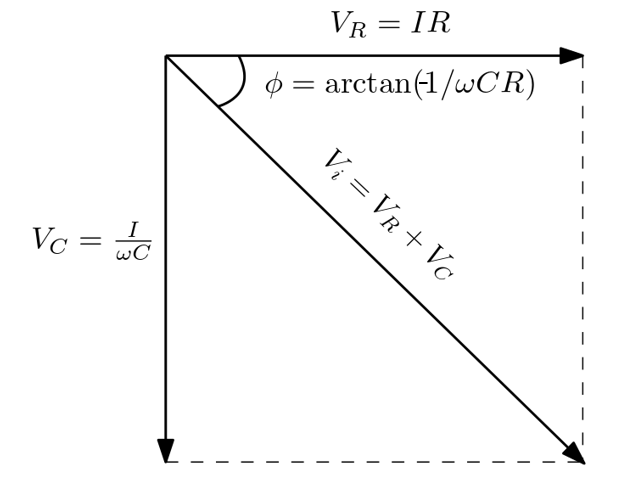
\includegraphics[width = 0.6\linewidth]{phys241_lab3_picture3.png}
				\captionsetup{margin=1cm}
				\caption{Vector diagram for Experiment $2$ involving $V_{R}$ and $V_{i}$ at frequency $f_{H}$. The diagram presented is to scale with $V_{R}$ = $V_{i}/\sqrt{2}$. We also note from the figure that $V_{R}$ lags $V_{i}$ since $\phi < 0$.}
			\end{figure}
		\section*{Question 5.}
			The channel 1 waveform increased as a result of adding a DC offset, whilst the channel 2 waveform remained unchanged. This is explained by the setup employed experimentally. All the DC voltage goes to charging the capacitor and so it is read by channel 1. The channel 2 is at position $V_{R}$ so nothing will change at that point for the latter reason. 
		\section*{Question 6.}
			\begin{figure}[H]
				\centering
				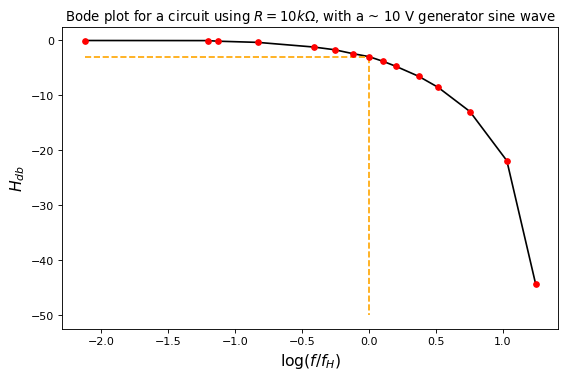
\includegraphics[width= 0.9\linewidth]{phys241_lab3_picture4.png}
				\captionsetup{margin=1cm}
				\caption{Bode plot for Experiment 4. The dotted lines indicate the $3$ db point.}
			\end{figure}
			It was found experimentally from the difference between the waves on the scope that the phase difference is $\phi = 70 ^\circ$, along with the cut-off frequency $f_{h} = 44 300 \ \si{\hertz}$. 
			
			From this we can immediately compute the inductance $L$ , 
			\begin{gather*}
				f_{h} = \frac{R}{2\pi L } \implies L = \frac{R}{(f_{h}2\pi )} = \frac{10 000 \ \si{\ohm}}{44300 \ \si{\hertz} 2\pi} = 0.036 \ H.
			\end{gather*}
		\section*{Question 7.}
		Due to the given configurations in which Experiment 1 to Experiment 4 are presented, along with their respective bode plots studied, we may conclude that 
			\begin{enumerate}
			\centering
				\item Experiment 1 is High-Pass 
				\item Experiment 2 is Low-Pass
				\item Experiment 3 is Low-Pass
				\item Experiment 4 is High-Pass
			\end{enumerate}
			
		\appendix
		\section*{Appendix}
		\begin{table}[h]
		\centering
		\caption{
		Experimental data gathered for construction of the bode plots presented in Figure 2 and Figure 4.
		}
		\begin{tabular}{cccc}
		\toprule
		\toprule
		\multicolumn{4}{c}{Raw Data} \\
		\multicolumn{2}{c}{Experiment 2} & \multicolumn{2}{c}{Experiment 4}\\
		\cmidrule(lr){1-2} \cmidrule(l){3-4}
		Frequency($f$) & Amplitude Ratio & Frequency($f$) & Amplitude Ratio\\
		$[\si{\kilo\hertz}]$ & & $[\si{\kilo\hertz}]$ & \\
		\midrule
		$0.03$ & $0.0068$ & $5.3$ & $0.990$ \\
		$0.05$ & $0.0110$ & $13.3$ & $0.988$ \\
		$0.10$ & $0.0468$ & $14.3$ & $0.976$ \\
		$0.20$ & $0.0980$ & $19.3$ & $0.952$ \\
		$0.60$ & $0.386$ & $29.3$ & $0.864$ \\
		$1.00$ & $0.580$ & $34.3$ & $0.816$ \\
		$1.40$ & $0.707$ & $39.3$ & $0.752$ \\
		$1.80$ & $0.78$ & $44.3$ & $0.707$ \\
		$2.20$ & $0.84$ & $49.3$ & $0.64$ \\
		$2.60$ & $0.88$ & $54.3$ & $ 0.576$ \\
		$3.00$ & $0.904$ & $64.3$ & $ 0.468$ \\
		$4.00$ & $0.952$ & $74.3$ & $ 0.372$ \\
		$8.00$ &  $0.996$ & $94.3$ & $0.224$ \\
		$10.00$ & $1.005$ & $12.43$ & $0.08$ \\
		 & & $15.43$ & $0.006$ \\
		\bottomrule
		\bottomrule
		\end{tabular}
		\end{table}
	\end{document}